\subsubsection{\stid{1.13} Argobots: Flexible, High-Performance Lightweight Threading }

\paragraph{Overview}

Efficiently supporting massive on-node parallelism demands highly
flexible and lightweight threading and tasking runtimes. At the
sametime, existing lightweight abstractions have shortcomings while
delivering generality and specialization.  Our group at Argonne
developed a lightweight, low-level threading and tasking framework,
called Argobots.  The key focus areas of this project are: (1) To
provide a framework that offers powerful capabilities for users to
allow efficient translation of high-level abstractions to low-level
implementations. (2) To provide interoperability with other
programming systems such as OpenMP and MPI as well as with other
software components (e.g., I/O services). (3) To provide a programming
framework that manages hardware resources more efficiently and reduce
interference with colocated applications.

\paragraph{Key Challenges}

Several user-level threading and tasking models have been proposed in
past to address the shortcomings of OS-leve threads, primarily with
respect to cost and flexibility. Their lightweight nature and flexible
generic interface play an important role at managing efficiently the
massive concurrency expected at the Exascale level.  Existing
user-level threading and tasking models, however, are either too
specific to applications or architectures or are not as powerful or
flexible. Existing runtimes tailored for generic use \cite{GNUPth,
  PLDI97_Taura, COSET05_Thibault, COB14_Nakashima, MTAAP08_Wheeler,
  PPoPP99_Taura, SenSys06_Dunkels, TBB1, EuroPar08_Perache} are
suitable as common frameworks to facilitate portability and
interoperability but offer insufficient flexibility to efficeintly
capture higher-level abstractions, while specialized runtimes
\cite{ATC02_Adya, SolarisThreads, SOSP03_von_Behren, StateThreads,
  PLDI07_Li, MTAAP09_Porterfield, WMPP05_Cuvillo, IntelOMP, Nanos++,
  LCPC96_Kale, PACT14_Treichler} are tailored to specific environment.

\paragraph{Solution Strategy}

Argobots offers a carefully designed execution model that balances
generality of functionality with providing a rich set of controls to
allow specialization by end users or high-level programming models
\cite{seo2018}.  Delivering high performance in Argobots while
providing a rich set of capabilities is achieve by heavily optimizing
critical paths as well as by exposing configuration knobs and a rich
API that allow users to trim unnecessary costs. Furthermore, Argobots
honors high degrees of expressibility through three key aspects:

\begin{enumerate}

\item Capturing the requirements of different \emph{work units}, which
are the most basic manageable entities. Work units that require
private stacks and context-saving capabilities, referred to as
\textit{user-level threads} (ULTs, also called \textit{coroutines} or
\textit{fibers}), are fully fledged threads usable in any context.
\emph{Tasklets} do not require private stacks. They are more
lightweight than ULTs because they do not incur context saving and
stack management overheads.  Tasklets, however, are restrictive; they
can be executed only as atomic work units that run to completion
without context switching.

\item Exposing hardware computational units through \emph{execution
streams} as OS-level threads to execute work units. Unlike existing
generic runtimes, ESs are exposed to and manageable by users.

\item Allowing full control over \emph{work unit management}.  Users
can freely manage \emph{scheduling} and mapping of work units to ESs
through \emph{thread pool} management, and thus achieving the desired
behavior. Figure~\ref{fig:sollve-argobots} illustrates the various
building blocks in the Argobots framework and the interactions between
them to build a hypothetical system.

\end{enumerate}

\begin{figure}[htb]
  \centering
  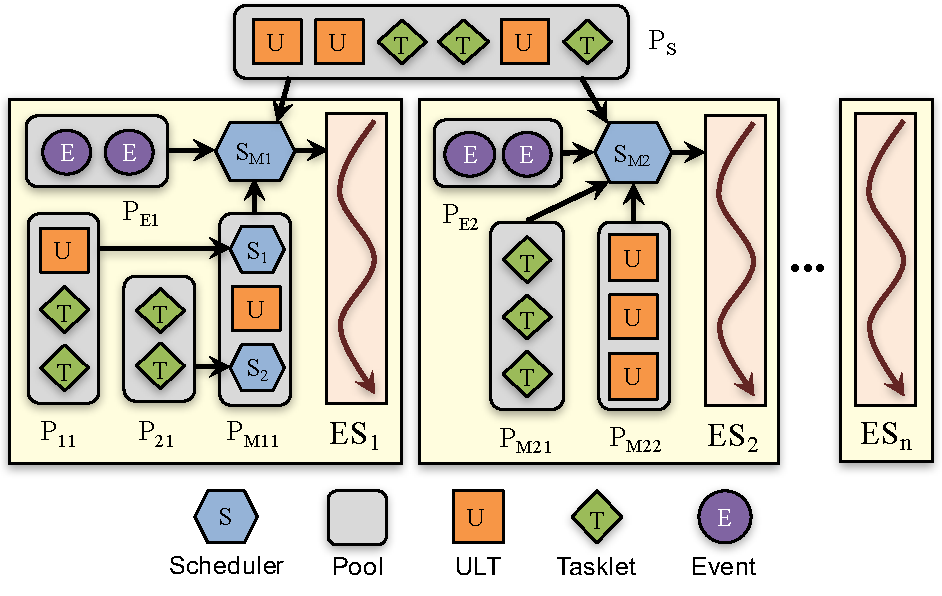
\includegraphics[height=3in]{projects/2.3.1-PMR/2.3.1.13-SOLLVE/SOLLVE-ARGOBOTS.pdf}
  \caption{\label{fig:sollve-argobots}Argobots execution model}
\end{figure}


\paragraph{Recent Progress}

Argobots was built from the ground up focusing on fast critical paths
and a flexibly API. Several programming systems, such as OpenMP, Cilk,
and Charm++, have been demonstrated to run efficiently using Argobots
as their underlying threading layer. Our most recent successful
integration is our BOLT OpenMP runtime that demonstrated significant
improvements over commercial and open source production OpenMP
runtimes. Furthermore, composing multiple programming systems or
libraries proved to be more efficient using Argobots as the
interoperation layer as opposed to a OS-level interaction. This was
demonstrated by achieving performance when multiple application
threads access the MPI stack or when applications are collocated I/O
services that incur significant overheads to deliver high response
times.

Argobots featured three software releases and publications in top tier
venues in the field. It has been recently extended with new thread
management techniques, called \emph{dynamic promotion}, that adapt to
application needs in terms of suspension as an alternative to
user-hinted distinction between work units. This effectively improves
user productivity while relying on runtime adaptation to deliver high
performance~\cite{iwasaki2018}. Recently, the Argobots API was also
extended to facilitate better resource utilization under idleness, has
been hadned with performance optimizations and stabilization, and
experienced improvements in the debugging infrastructure.

\paragraph{Next Steps}

Argobots continues to grow in terms of features, integration or
composition with other systems, and hardening. Below is a short
list of the major ongoing and planned extensions and optimizations.

\begin{enumerate}

\item Extend and optimize Argobots for BOLT needs. While Argobots is
used by several systems, BOLT is one of those that rely heavily on
Argobots to perform well and offer necessary abstractions. We plan to
continue involving Argobots in our BOLT optimization process and
extend Argobots and optimize it accordingly.

\item Investigating composition challenges and opportunities outside
MPI. Our investigation of using Argobots as the interoperability layer
between heterogeneous software systems involved mostly MPI (given its
prominence) and I/O services to some extent. This investigation is
only preliminary; several HPC programming systems and libraries rely
on OS-level threads and their composition might benefit for Argobots
and warrants investigation.

\end{enumerate}
